\newcommand{\svrname}{Mr Thomas Rees}
\newcommand{\jkfside}{oneside}
\newcommand{\jkfhanded}{right}

\newcommand{\studentname}{Harry Langford}
\newcommand{\studentemail}{hjel2@cam.ac.uk}

\documentclass[10pt,\jkfside,a4paper]{article}

\newcommand{\svcourse}{CST Part IA: Software Engineering and Security}
\newcommand{\svnumber}{1}
\newcommand{\svvenue}{Microsoft Teams}
\newcommand{\svdate}{2022-05-11}
\newcommand{\svtime}{15:00}
\newcommand{\svuploadkey}{CBd13xmL7PC1zqhNIoLdTiYUBnxZhzRAtJxv/ytRdM1r7qIfwMsxeVwM/pPcIo8l}

\newcommand{\svrname}{Dr Sam Ainsworth}
\newcommand{\jkfside}{oneside}
\newcommand{\jkfhanded}{yes}

\newcommand{\studentname}{Harry Langford}
\newcommand{\studentemail}{hjel2@cam.ac.uk}

% DO NOT add \usepackage commands here.  Place any custom commands
% into your SV work files.  Anything in the template directory is
% likely to be overwritten!

\usepackage{fancyhdr}

\usepackage{lastpage}       % ``n of m'' page numbering
\usepackage{lscape}         % Makes landscape easier

\usepackage{verbatim}       % Verbatim blocks
\usepackage{listings}       % Source code listings
\usepackage{epsfig}         % Embed encapsulated postscript
\usepackage{array}          % Array environment
\usepackage{qrcode}         % QR codes
\usepackage{enumitem}       % Required by Tom Johnson's exam question header

\usepackage{hhline}         % Horizontal lines in tables
\usepackage{siunitx}        % Correct spacing of units
\usepackage{amsmath}        % American Mathematical Society
\usepackage{amssymb}        % Maths symbols
\usepackage{amsthm}         % Theorems

\usepackage{ifthen}         % Conditional processing in tex

\usepackage[top=3cm,
            bottom=3cm,
            inner=2cm,
            outer=5cm]{geometry}

% PDF metadata + URL formatting
\usepackage[
            pdfauthor={\studentname},
            pdftitle={\svcourse, SV \svnumber},
            pdfsubject={},
            pdfkeywords={9d2547b00aba40b58fa0378774f72ee6},
            pdfproducer={},
            pdfcreator={},
            hidelinks]{hyperref}


% DO NOT add \usepackage commands here.  Place any custom commands
% into your SV work files.  Anything in the template directory is
% likely to be overwritten!

\usepackage{fancyhdr}

\usepackage{lastpage}       % ``n of m'' page numbering
\usepackage{lscape}         % Makes landscape easier

\usepackage{verbatim}       % Verbatim blocks
\usepackage{listings}       % Source code listings
\usepackage{graphicx}
\usepackage{float}
\usepackage{epsfig}         % Embed encapsulated postscript
\usepackage{array}          % Array environment
\usepackage{qrcode}         % QR codes
\usepackage{enumitem}       % Required by Tom Johnson's exam question header

\usepackage{hhline}         % Horizontal lines in tables
\usepackage{siunitx}        % Correct spacing of units
\usepackage{amsmath}        % American Mathematical Society
\usepackage{amssymb}        % Maths symbols
\usepackage{amsthm}         % Theorems

\usepackage{ifthen}         % Conditional processing in tex

\usepackage[top=3cm,
            bottom=3cm,
            inner=2cm,
            outer=5cm]{geometry}

% PDF metadata + URL formatting
\usepackage[
            pdfauthor={\studentname},
            pdftitle={\svcourse, SV \svnumber},
            pdfsubject={},
            pdfkeywords={9d2547b00aba40b58fa0378774f72ee6},
            pdfproducer={},
            pdfcreator={},
            hidelinks]{hyperref}

\renewcommand{\headrulewidth}{0.4pt}
\renewcommand{\footrulewidth}{0.4pt}
\fancyheadoffset[LO,LE,RO,RE]{0pt}
\fancyfootoffset[LO,LE,RO,RE]{0pt}
\pagestyle{fancy}
\fancyhead{}
\fancyhead[LO,RE]{{\bfseries \studentname}\\\studentemail}
\fancyhead[RO,LE]{{\bfseries \svcourse, SV~\svnumber}\\\svdate\ \svtime, \svvenue}
\fancyfoot{}
\fancyfoot[LO,RE]{For: \svrname}
\fancyfoot[RO,LE]{\today\hspace{1cm}\thepage\ / \pageref{LastPage}}
\fancyfoot[C]{\qrcode[height=0.8cm]{\svuploadkey}}
\setlength{\headheight}{22.55pt}


\ifthenelse{\equal{\jkfside}{oneside}}{

 \ifthenelse{\equal{\jkfhanded}{left}}{
  % 1. Left-handed marker, one-sided printing or e-marking, use oneside and...
  \evensidemargin=\oddsidemargin
  \oddsidemargin=73pt
  \setlength{\marginparwidth}{111pt}
  \setlength{\marginparsep}{-\marginparsep}
  \addtolength{\marginparsep}{-\textwidth}
  \addtolength{\marginparsep}{-\marginparwidth}
 }{
  % 2. Right-handed marker, one-sided printing or e-marking, use oneside.
  \setlength{\marginparwidth}{111pt}
 }

}{
 % 3. Alternating margins, two-sided printing, use twoside.
}


\setlength{\parindent}{0em}
\addtolength{\parskip}{1ex}

% Exam question headings, labels and sensible layout (courtesy of Tom Johnson)
\setlist{parsep=\parskip, listparindent=\parindent}
\newcommand{\examhead}[3]{\section{#1 Paper #2 Question #3}}
\newenvironment{examquestion}[3]{
\examhead{#1}{#2}{#3}\setlist[enumerate, 1]{label=(\alph*)}\setlist[enumerate, 2]{label=(\roman*)}
\marginpar{\href{https://www.cl.cam.ac.uk/teaching/exams/pastpapers/y#1p#2q#3.pdf}{\qrcode{https://www.cl.cam.ac.uk/teaching/exams/pastpapers/y#1p#2q#3.pdf}}}
\marginpar{\footnotesize \href{https://www.cl.cam.ac.uk/teaching/exams/pastpapers/y#1p#2q#3.pdf}{https://www.cl.cam.ac.uk/\\teaching/exams/pastpapers/\\y#1p#2q#3.pdf}}
}{}


\usepackage{graphicx}
\graphicspath{ {./images/} }
\usepackage{enumitem}

\begin{document}

\begin{enumerate}[label=(\alph*)]

\item Explain why understanding the human vision system is important in graphics, 
and give some examples of where graphics has been affected by the limits of human 
vision.

Human vision is imperfect. The most obvious example of this is our colour vision: since 
humans can only see electromagnetic waves with wavelengths between $400nm$ and $700nm$ 
there is no point of rendering in colours outside those frequencies (such as in UV or in 
Infrared) as the human eye will not be able to detect them. Hence the colour gamuts which 
are used in renderering is constrained by the human colour gamut (although compared to 
the human eye's colour gamut; most gamuts are not close to reaching this constraint).

Human colour vision is defined by three types of cells -- which all percieve different 
colours. Short Cone Cells, Medium Cone Cells and Long Cone Cells: Short Cone Cells 
can view blue light (and other short-wavelength colours); Medium Cone Cells can 
see green light (and other medium-wavelength colours); and Long Cone Cells 
can see red light and other long-wavelength colours. 
To mimick this on a computer, colours are usually divided into RGB components.

Since human colour vision is imperfect, there are many colours which although distinct 
are totally indistinguishable to the human eye (known as metamers). Graphics has hence 
been unable to use those colours in conjunction and in general steps have been taken 
in different colour specifications to ensure that metamers are not represented (to maximise 
the number of distinct colours). For example being able to represent 20 different greens 
which were indistinguishable would be wasteful.

Some people are colourblind: to account for this, good GUI's should not rely only on 
colours to indicate the differences between things. For example two buttons indicating 
``yes'' and ``no'' should not differently coloured but otherwise identical (ie simply 
red and green) since that would cause difficulty to people who suffered from red-green 
colour blindness.

The human eye also has a limited resolution: there exists a point beyond which it is 
pointless to render at a higher resolution. This has affected, for example, cinema's: 
The resolution on cinema screens is very low. For example, a laptop typically has a 
resolution thousands of times that of a cinema screen. However since the cinema screen 
is so large and people sit so far away from it compared to a laptop; the low resolution 
is not problematic. If human vision was significantly better then cinemas would have to 
purchase higher resolution (and more expensive) screens to account for this. The 
existence of higher resolution screens would also mean filmmakers would need to film in 
higher resolution -- again using more expensive equipment, more expensive rendering and 
CGI.

In more usual applications, since humans have varied quality of vision, GUI's 
should always offer accessibility features such as larger text or text-to-speech.

The pupil in the human eye does not have a zero diameter. This means that the human eye 
is similar a finite aperature camera. So when we focus on things in the foreground, things in 
the background become blurry and vice versa. When rendering, we should try to take account 
of this by using Depth of Field rendering to create a focus and slightly blur things which 
we are not focussing on to the same extent as is natural for the human eye. This helps to 
make renders more realistic.

Humans, in general, have two eyes and hence have a wide field of view. As such, screens 
and monitors are landscape and have a wide field of view comparable to that of humans.

\item Why is it better to look at faint stars and comets slightly off-centre rather 
than looking directly at them?

The human eye has two main types of cells which detect light -- rod cells and cone cells 
(there are a further three subcategories of cone cells however, they're not relevant for 
this question so I'll omit them). Rod cells are used to view low light environments however do 
not give colour vision and while Cone cells are used to view colours. In the fovea (the centre 
of the eye -- the point on the retina with the highest density of cone cells), there are no rod cells.

This means that the center of the eye cannot see faint items as well (however has much better 
colour vision). If you look directly at faint stars; then cone cells cannot detect them well since 
they are so dim and since there are no rod cells in the centre of your eye, they do not detect them. 
This means that your vision of the faint stars is very poor if you look at them straight on.

While, if you look at the faint stars and comets slightly off-centre then you are not using the fovea -- 
and these parts of the eye do have a significantly higher amount of rod cells -- so they can detect 
the dim light from the stars much better and hence see them better.

\item In a CAD system using blue lines on a black background would be a poor choice for 
the interface colours for designing an object. Why is this?

The human eye is less sensitive to lower wavelenths -- such as blues compared to other colours. 
This means that blues do not ``stand out'' much. So using blue lines on a black background would 
make it very difficult for humans to see the lines. The purpose of a CAD system is to make design 
easier -- and making the UI difficult to see goes against this. Hence using blue lines on a black 
background would be a poor choice of interface colours.

\item Calculate the ultimate monitor resolution (i.e. colour pixels/inch) beyond which 
better resolution will be unnecessary. Hint: Try starting with experimental data on how 
`precise' our eyes are.

``Resolution'' is the smallest possible distance between two points such that we can see them to be different. 
I can discern (with glasses) the top and bottom of a letter ``A'' on a fire action sign on the other 
side of my room (about 5m away) -- these two points are around 1mm away from each other. Experimentally, humans 
seem to have a field of view about $160^o$ horizontally and around $90^o$ vertically. This is a third of the 
surface of a sphere. The surface area of a sphere with a radius of $5m$ is $4\cdot \pi \cdot 5^2m^3 \approx 314m^2$ 
Since the field of view of a human eye is a third that of the surface of a sphere: the human eye can see $~105m^2$. 
Since at a distance of $5m$, we can see one point in 1mm; we can see $1000^2 = 1000 000$ points per metre. So the 
resolution of the human eye is $\approx 104 \cdot 1000 000 = 104 000 000$. So the resolution of the human eye is 
around 100MP. And so the ultimate monitor resolution would be about 100MP -- although, given that monitors are often 
not more than 5\% - 10\% of our field of view, practically any resolution above 5MP or 10MP would be impossible to 
distinguish from the ultimate resolution.

\item \begin{examquestion}{2005}{6}{6}

\begin{enumerate}[label=(\alph*)]

\item  In ray tracing, once we have determined where a ray strikes an object, the
illumination at the intersection point can be calculated using the formula:

\begin{equation}
\begin{split}
I &= I_ak_a+\sum_{i}I_ik_d(\mathbf{L}_i\cdot \mathbf{N}) + \sum_{i}I_ik_s(\mathbf{R}_i\cdot \mathbf{V})^n.\\
\end{split}
\end{equation}

Explain what real effect each of the three terms is trying to model, how
accurately it models the real effect, and explain what each of the following
symbols means, within the context of this formula:

\begin{equation*}
\begin{split}
I, I_a, i, I_i, k_a, k_d, k_s, \mathbf{L}_i, \mathbf{N}, \mathbf{R}_i, \mathbf{V}, n\\
\end{split}
\end{equation*}

$I$ is the linear colour of the pixel after all illumination has been added.

$I_ak_a$ is called ambient illumination and is trying to model the background light in a scene. 
$I_a$ is the colour of the ambient light in the scene and $k_a$ is the diffuse colour of the surface -- 
attempting to model the absorbtion spectrum of the surface discretely.
It is (in most situations) a reasonable approximation -- usually even the darkest areas in an 
image are not pitch black due to light reflecting diffusely off other objects and eventually 
reaching most corners in a scene. However, this more realistic calculation would be incredibly 
expensive to perform and so it is appropriate to use ambient illumination as an approximation 
of this -- since even though it is not the same it gives a similar effect.

$\sum_{i}I_ik_d(\mathbf{L}_i\cdot \mathbf{N})$ is called diffuse illumination. It is trying to 
model incident light on a surface from each light source which reflects diffusely. It actually 
models this pretty accurately. For each light source in the image, it takes the colour of the 
light $i$ ($I_i$), multiplies it by the proportion of each component which is absorbed by the 
material ($k_d$ -- the diffuse colour of the surface multiplied by the diffuse colour of the 
surface) then multiplies it by the proportion of the light from the light source which is incident 
on the surface (after having ensured that there is no collision between the light and another object 
before reaching the pixel) (which is equal to the cosine of the angle between the normal at the surface and the 
surface [$\mathbf{N}$] and the unit vector in the direction of the light source [$\mathbf{L}_i$]). 
However: in reality the absorbtion spectrum is continuous while the absorbtion spectrum in this 
equation is only a discrete approximation of it.

$\sum_{i}I_ik_s(\mathbf{R}_i\cdot \mathbf{V})^n.$ is called specular illumination. 
$I_i$ is the light from light source $i$, $k_s$ is the specular colour of the object 
multiplied by the specular coefficient. $\mathbf{R}_i$ is the unit vector in the direction of the 
reflection of the vector from the light to the pixel in the normal to the surface at the pixel. 
$\mathbf{V}$ is the unit vector pointing to the camera. $n$ is the ``specular roughness'' of the object.
It attempts to 
model light which reflects specularly off of a surface giving a plastic-y ``gleam'' to the object. 
While this effect does exist -- it's very rare and only really happens to a meaningful extent on 
plastics and some metals. 
Neither of which are particularly common. Often in renderings, the specular coefficient of the surface 
is greatly overestimated leading to a lot of specular illumination which you just don't see normally. 
So although the model itself is reasonably appropriate, due to it's abuse and overuse I have to say that 
it doesn't accurately model the real effect.
\end{enumerate}

\end{examquestion}

\item Basic ray tracing uses a single sample per pixel. Describe four distinct 
reasons why one might use multiple samples per pixel. Explain the effect that each 
is trying to achieve, and outline the mechanism by which it achieves the effect.

\begin{itemize}
\item Multiple samples per pixel ensure that colour boundaries are soft -- leading 
to soft edges rather than jagged ones.
\item The colour of the area that the pixel represents may not be uniform -- taking multiple 
samples leads to a better representation of the colours of the pixel.
\item Multiple samples per pixel reduces the chance of missing small objects which do not cover 
the centre of any pixels.
\item Multiple samples per pixel reduces the chance of thin objects being split up into multiple 
pieces.
\end{itemize}

\item
\begin{examquestion}{1998}{4}{10} 

\begin{enumerate}[label=(\alph*)]

\item The diagram below represents a scene being ray traced. The circles may be 
taken to represent the cross-sections of spheres.

\begin{center}
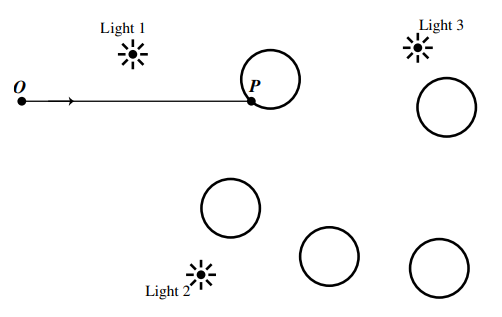
\includegraphics{diagram1998}
\end{center}

In answering the remaining parts of this question you may use the single sheet
supplied with the examination paper. Ensure that you attach it to the rest of your
answer.

A particular ray from the eyepoint O has been found to have its closest intersection
with an object at point P. Show, on a diagram, all subsequent rays and vectors
which must be found in order to calculate the shading at point P. Explain the
purpose of each one.

Assume that:

\begin{itemize}

\item Each object has ambient, diffuse and specular reflections, but is not a 
perfect reflector.

\item Each object is opaque.

\item All rays and vectors lie in the plane of the paper.

\item We are not using distributed ray tracing.

\end{itemize}

\vspace{1em}

Ambient illumination requires no rays or vectors to calculate, diffuse illumination requires the normal, 
the unit direction vector pointing to the light. Specular illumination requires the normal to the point, 
the unit directon vector pointing to the light, the unit vector in the direction of the reflection of the 
vector pointing towards the light in the normal and the vector pointing towards the observer.
In addition to these vectors, we require a ray from each light to the point to determine if light from 
that light intersects with anything before hitting the point.

So: to calculate the light on a single point, we need two vectors and an additional two vectors 
for each light which is in the scene (and is shining on the object).
The two vectors we need for every calculation are: the unit normal and the unit vector in the 
direction of the observer. The two vectors we need per light are: the unit vector pointing in the 
direction of the light from the point $P$ and a unit 
vector in the direction of the reflection of the incident light in the normal.

The unit normal is used to calculate the cosine of the angle between the unit vector in the 
direction of each light (which is included in the equation for diffuse illumination to account 
for the curves of the object. -- and to calculate the vector after the light has been reflected in the 
object. This reflected vector is (dotted with the unit vector in the direction of the observer and) 
used to work out the proportion of light which is refused specularly which goes to a specific 
college.

Since the spheres are not perfect reflectors we do not have to consider reflected rays.

\begin{center}
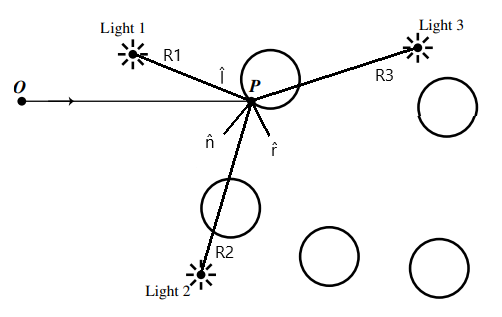
\includegraphics{diagram1998withrays}
\end{center}

$R1$ is the ray that is cast from the light 1 to determine whether it intersects any other spheres before reaching 
the point $P$. Since it does not intersect any other spheres, light will be cast from the light 1 on the point $P$.

$R2$ is the ray that is cast from the light 2 to determine whether the light intersects any other 
spheres before the point $P$. Since it does, light from the light 2 will not be cast on the point $P$.

$R3$ is the ray that is cast from the light 3 to determine whether the light intersects any spheres before reaching the 
point $P$. Since it intersects the sphere (but not at the point $P$), no light from light 3 will be cast on the point $P$.

$\hat n$ is the unit normal vector at the point $P$. This is used to calculate the reflection of the vector $R1$ 
in the point $P$: normalize$(\hat l - 2\cdot \hat n)$. It is also used to calculate the proportion of the light incident on the point $P$ which is 
perpendicular to the plane (by applying the dot product with $\hat l$).

$\hat l$ is the unit vector in the direction of the light R1. It is used as described above.

$\hat r$ is the reflection of the vector from the light to the point $P$ ($\hat l$) in the normal $\hat n$. 
It is used to determine the specular illumination at that point.

\item Assume now that all of the objects are perfect reflectors (in addition to 
having ambient, diffuse and specular reflection). Show, on a separate diagram, 
the extra rays which need to be calculated and explain the purpose of each one.

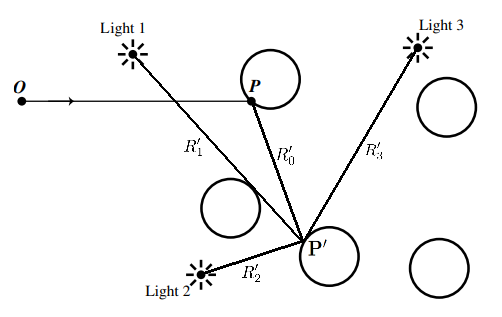
\includegraphics{diagram1998reflections}

We have to cast a ray $R_0$ from $P$ in the direction of the reflection of the ray incident on $P$ from the observer. 
This is to work out which point (if any) should be in the reflection at $P$. This ray hits another sphere at the point $P'$. 
We then have to calculate the illumination at the point $P'$. This involves casting a ray from each of the point light sources to 
the point $P'$ to determine if they intersect anything before hitting the point $P'$. So we have to cast three more rays, $R_1$, 
$R_2$ and $R_3$ -- one for each light source.

\end{enumerate}

\end{examquestion}

\end{enumerate}

\end{document}

